
%(BEGIN_QUESTION)
% Copyright 2008, Tony R. Kuphaldt, released under the Creative Commons Attribution License (v 1.0)
% This means you may do almost anything with this work of mine, so long as you give me proper credit

Determine what will happen to the following voltage drops (between specified test points in the circuit) if the resistance of resistor $R_2$ happens to increase:

$$\includegraphics[width=15.5cm]{i02915x01.eps}$$

\begin{itemize}
\item{} $V_{AC}$ = ({\it increase}, {\it decrease}, or {\it stay the same})
\vskip 10pt
\item{} $V_{BE}$ = ({\it increase}, {\it decrease}, or {\it stay the same})
\vskip 10pt
\item{} $V_{AD}$ = ({\it increase}, {\it decrease}, or {\it stay the same})
\vskip 10pt
\item{} $V_{CD}$ = ({\it increase}, {\it decrease}, or {\it stay the same})
\end{itemize}

\vfil 

\underbar{file i02915}
\eject
%(END_QUESTION)





%(BEGIN_ANSWER)

This is a graded question -- no answers or hints given!

%(END_ANSWER)





%(BEGIN_NOTES)

\begin{itemize}
\item{} $V_{AC}$ = {\bf decrease}
\vskip 10pt
\item{} $V_{BE}$ = {\bf decrease}
\vskip 10pt
\item{} $V_{AD}$ = {\bf stay the same}
\vskip 10pt
\item{} $V_{CD}$ = {\bf increase}
\end{itemize}

A good problem-solving technique to use here is imagining an {\it absolute} failure.  Instead of merely considering the effects of a resistance changing slightly, imagine that resistance suffering an extreme change (e.g. an increasing resistance gets viewed as an ``open,'' while a decreasing resistance gets viewed as a dead short).  Things are generally a little easier to analyze under such extreme conditions, and the directions of the changes in a linear DC circuit such as this will be the same as for a mild(er) fault.

%INDEX% Electronics review: qualitative analysis of DC series-parallel resistor circuit

%(END_NOTES)


